\section{Details of Multitenancy Stress Tests}
\label{appendix:multitenancy}

In multitenancy tests we are interested in examining the behavior of the systems under heavy and dynamic query load.
This simulates a common deployment in which the Accumulo cluster is a shared resource backing a group of application servers.
The benchmark service acts as our application server, receiving the full query result-set and producing a digested view for the client.
We’ve formulate this test to make the Accumulo cluster and its \texttt{SimpleFeature} index the only contested resource.

\subsection{Summary}

\subsubsection{GDELT}

Under heavy dynamic query load against a GDELT store, GeoWave is better able to cope with high concurrent load producing stable and predictable performance.
In our specific scenario it is able to process a $3.5$x higher request volume than GeoMesa.
We also found that GeoWave's return times increase roughly $1.5$ times faster than GeoMesa's as the size of the result set increases.
On the other hand, GeoMesa's return times increase roughly $8.5$ times faster than GeoWave's as the number of concurrent queries rises.
Additionally during this testing we have witnessed two instances where GeoMesa clusters entered degraded performance mode, where query duration seems to
increase permanently after a round of load testing.
We have not attempted to diagnose this issue but its effects are illustrated in our results.

{\bf Failure Analysis.}
The performance gap is further compounded because GeoWave is able to consistently complete queries covering large temporal spans ($12$ to $14$ months) before the $60$s client timeout.
When this does not happen the client connection times out and a new query is issued, which then must compete for resources with still executing scans.
Higher client timeouts cause the GeoMesa cluster to work under higher concurrent random scan load than GeoWave.
Highly concurrent random access scans cause tablet contention which is known to dramatically impact Accumulo performance.
This timeout cascade can be mitigated in deployment by tuning the allowed query load, cluster size, or canceling the scans when the client timeout happens.
Our benchmark services do not implement cancel-able queries so we are not able to comment on the difficulty of implementing such a feature.

\subsubsection{Generated Tracks}

Generated tracks load tests allows us to test the performance of GeoMesa XZ3 vs GeoWave tiered Hilbert index.
Under heavy load with variance both over spatial and temporal selectivity both GeoMesa and GeoWave produced stable and reliable performance.
GeoWave delivers $60$\% higher request completion volume vs GeoMesa with $95$th percentile response time being $7.5$s.


\subsection{Test Setup}

All queries are triggered by Gatling load-testing tool (\url{http://gatling.io}) issuing HTTP requests against a load-balanced group of application servers.
Gatling allows us to keep the number of active concurrent query connections constant.
A connection is considered active until the benchmark services iterates over the query results set or a time-out of $60$ seconds.

As with other tests the benchmark service saves the query timings, which happens even in the event of a time-out on the client/benchmark-server connection.
However, unlike the earlier test-ups all the queries per scenario are done against either GeoMesa or GeoWave - not both.
This produces a reliable and uninterrupted load on the target system.

\subsection{GDELT Test}

The queries are executed against GDELT ingested into a cluster with $5$ workers as in previous tests.
We reuse the City Buffers queries, as well as the queries against South American countries, randomly selecting parameters for spatial and temporal bounds.
Up to eight concurrent connections for each query group will be open with no pause between subsequent requests.
This is a very dynamic load test as the City Buffers  queries span up fourteen months and the South America queries will issue twelve \texttt{DataStore} queries for every HTTP request.

Because the Accumulo-backed \texttt{DataStore} can receive records from multiple tablet servers the application server network interface can easily become saturated.
These simulations increase the number of application servers relative to other tests to remove this bottle-neck and increase the query throughput until the cluster under test becomes the limiting resource.
Because small client queries trigger large query workloads we do not consider the connection between application server and Gatling client a limited resource.

\subsubsection{Test Results}

We are interested in how concurrency impacts the duration of query execution.
The number of concurrent queries at the time of submission is calculated based on query start and end times as recorded by the application service.
Before each round of testing we verified that all clusters were idle, not undergoing any compactions or scans.

{\bf Configuration 1: A Single Application Server.}
This configuration is expected to degenerate; a single application server does not have the network bandwidth to pull the requested records and we see query duration spike well past usual levels.
From the client perspective this scenario produced cumulative timeout rates of about $50$\% for both systems.
After this round of testing GeoMesa cluster experienced an unexpected severity of degradation in query performance.
This prompted us to bring up two replacements for future tests.
\begin{figure}[h!tb]
  \centering
  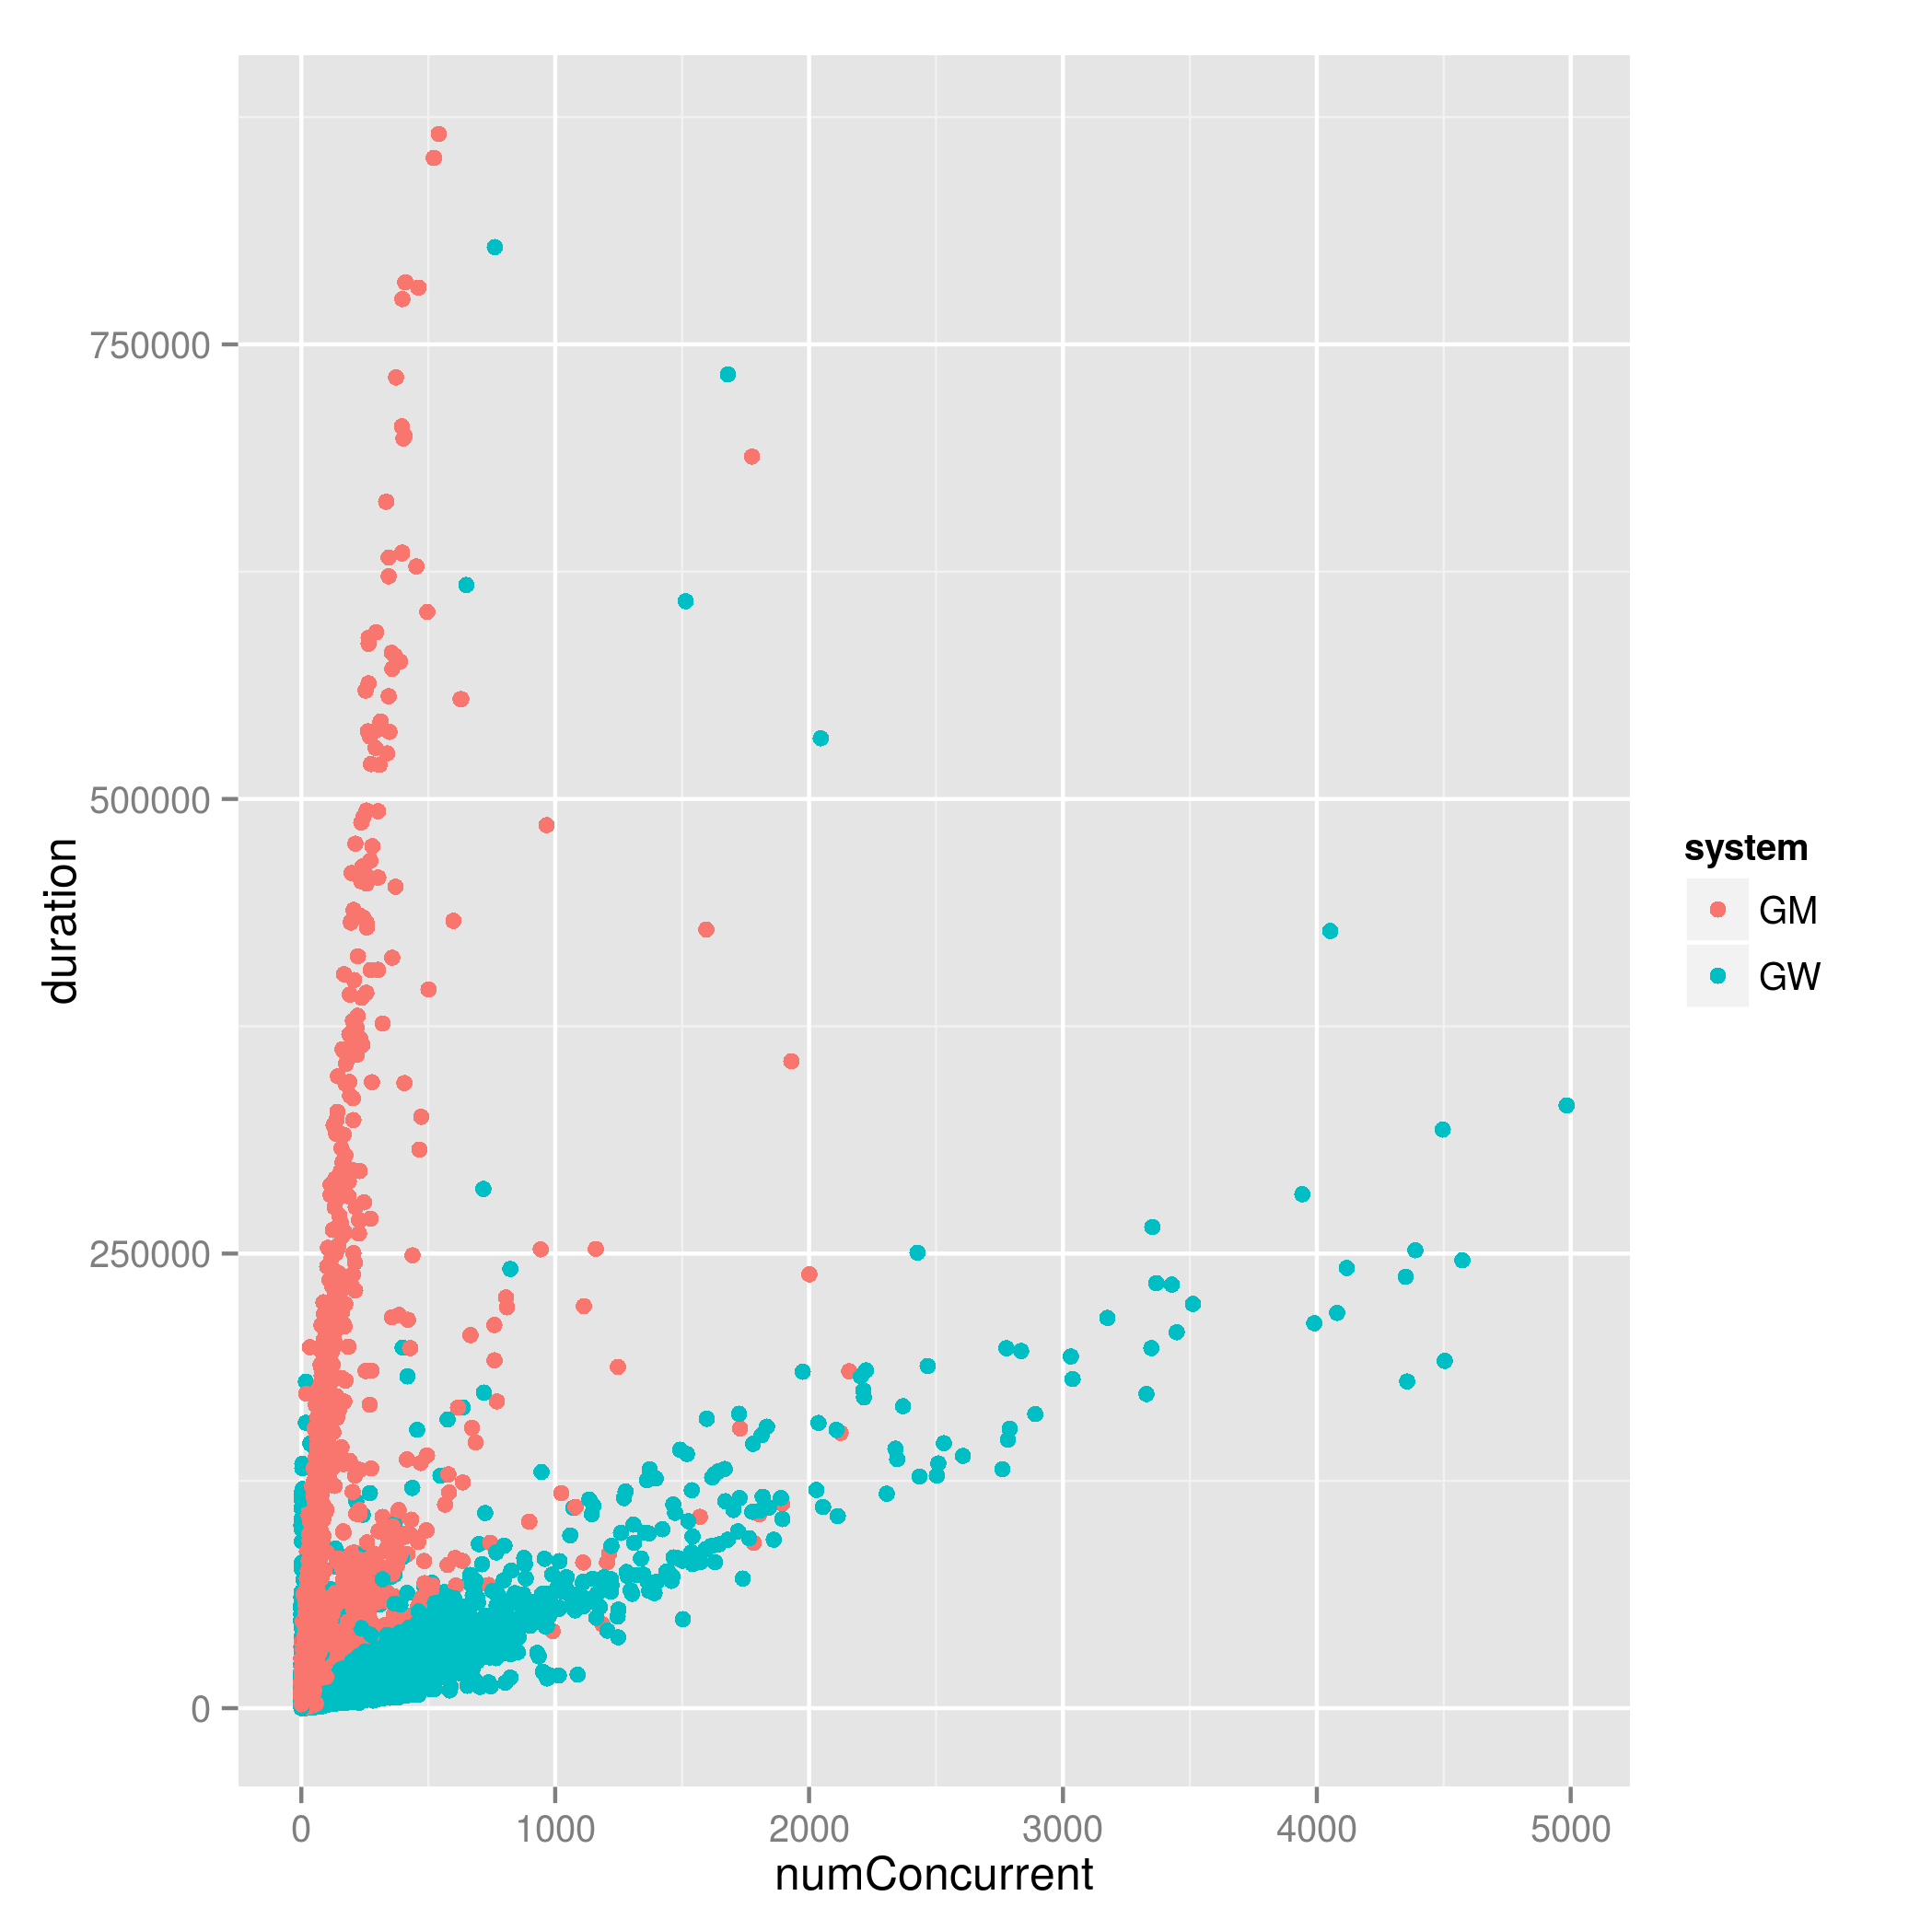
\includegraphics[width=0.60\textwidth]{../docs/img/multitenancy/graph_uncut_mt1.png}
  \caption{Results for configuration 1.}
  \label{config1}
\end{figure}

{\bf Configuration 2: 4 Application Servers.}
With four application servers we expect the network to no longer constrain the query execution. Notably we see that GeoMesa is working against higher concurrency and producing higher delays.
These effects are likely mutually-reinforcing.
From the client we saw the query timeouts drop to about $5$\% for GeoWave and remain at about $20$\% for GeoMesa.
These results contain two GeoMesa clusters and we do not see the effects of performance degradation from the \texttt{MT1} test.
\begin{figure}[h!tb]
  \centering
  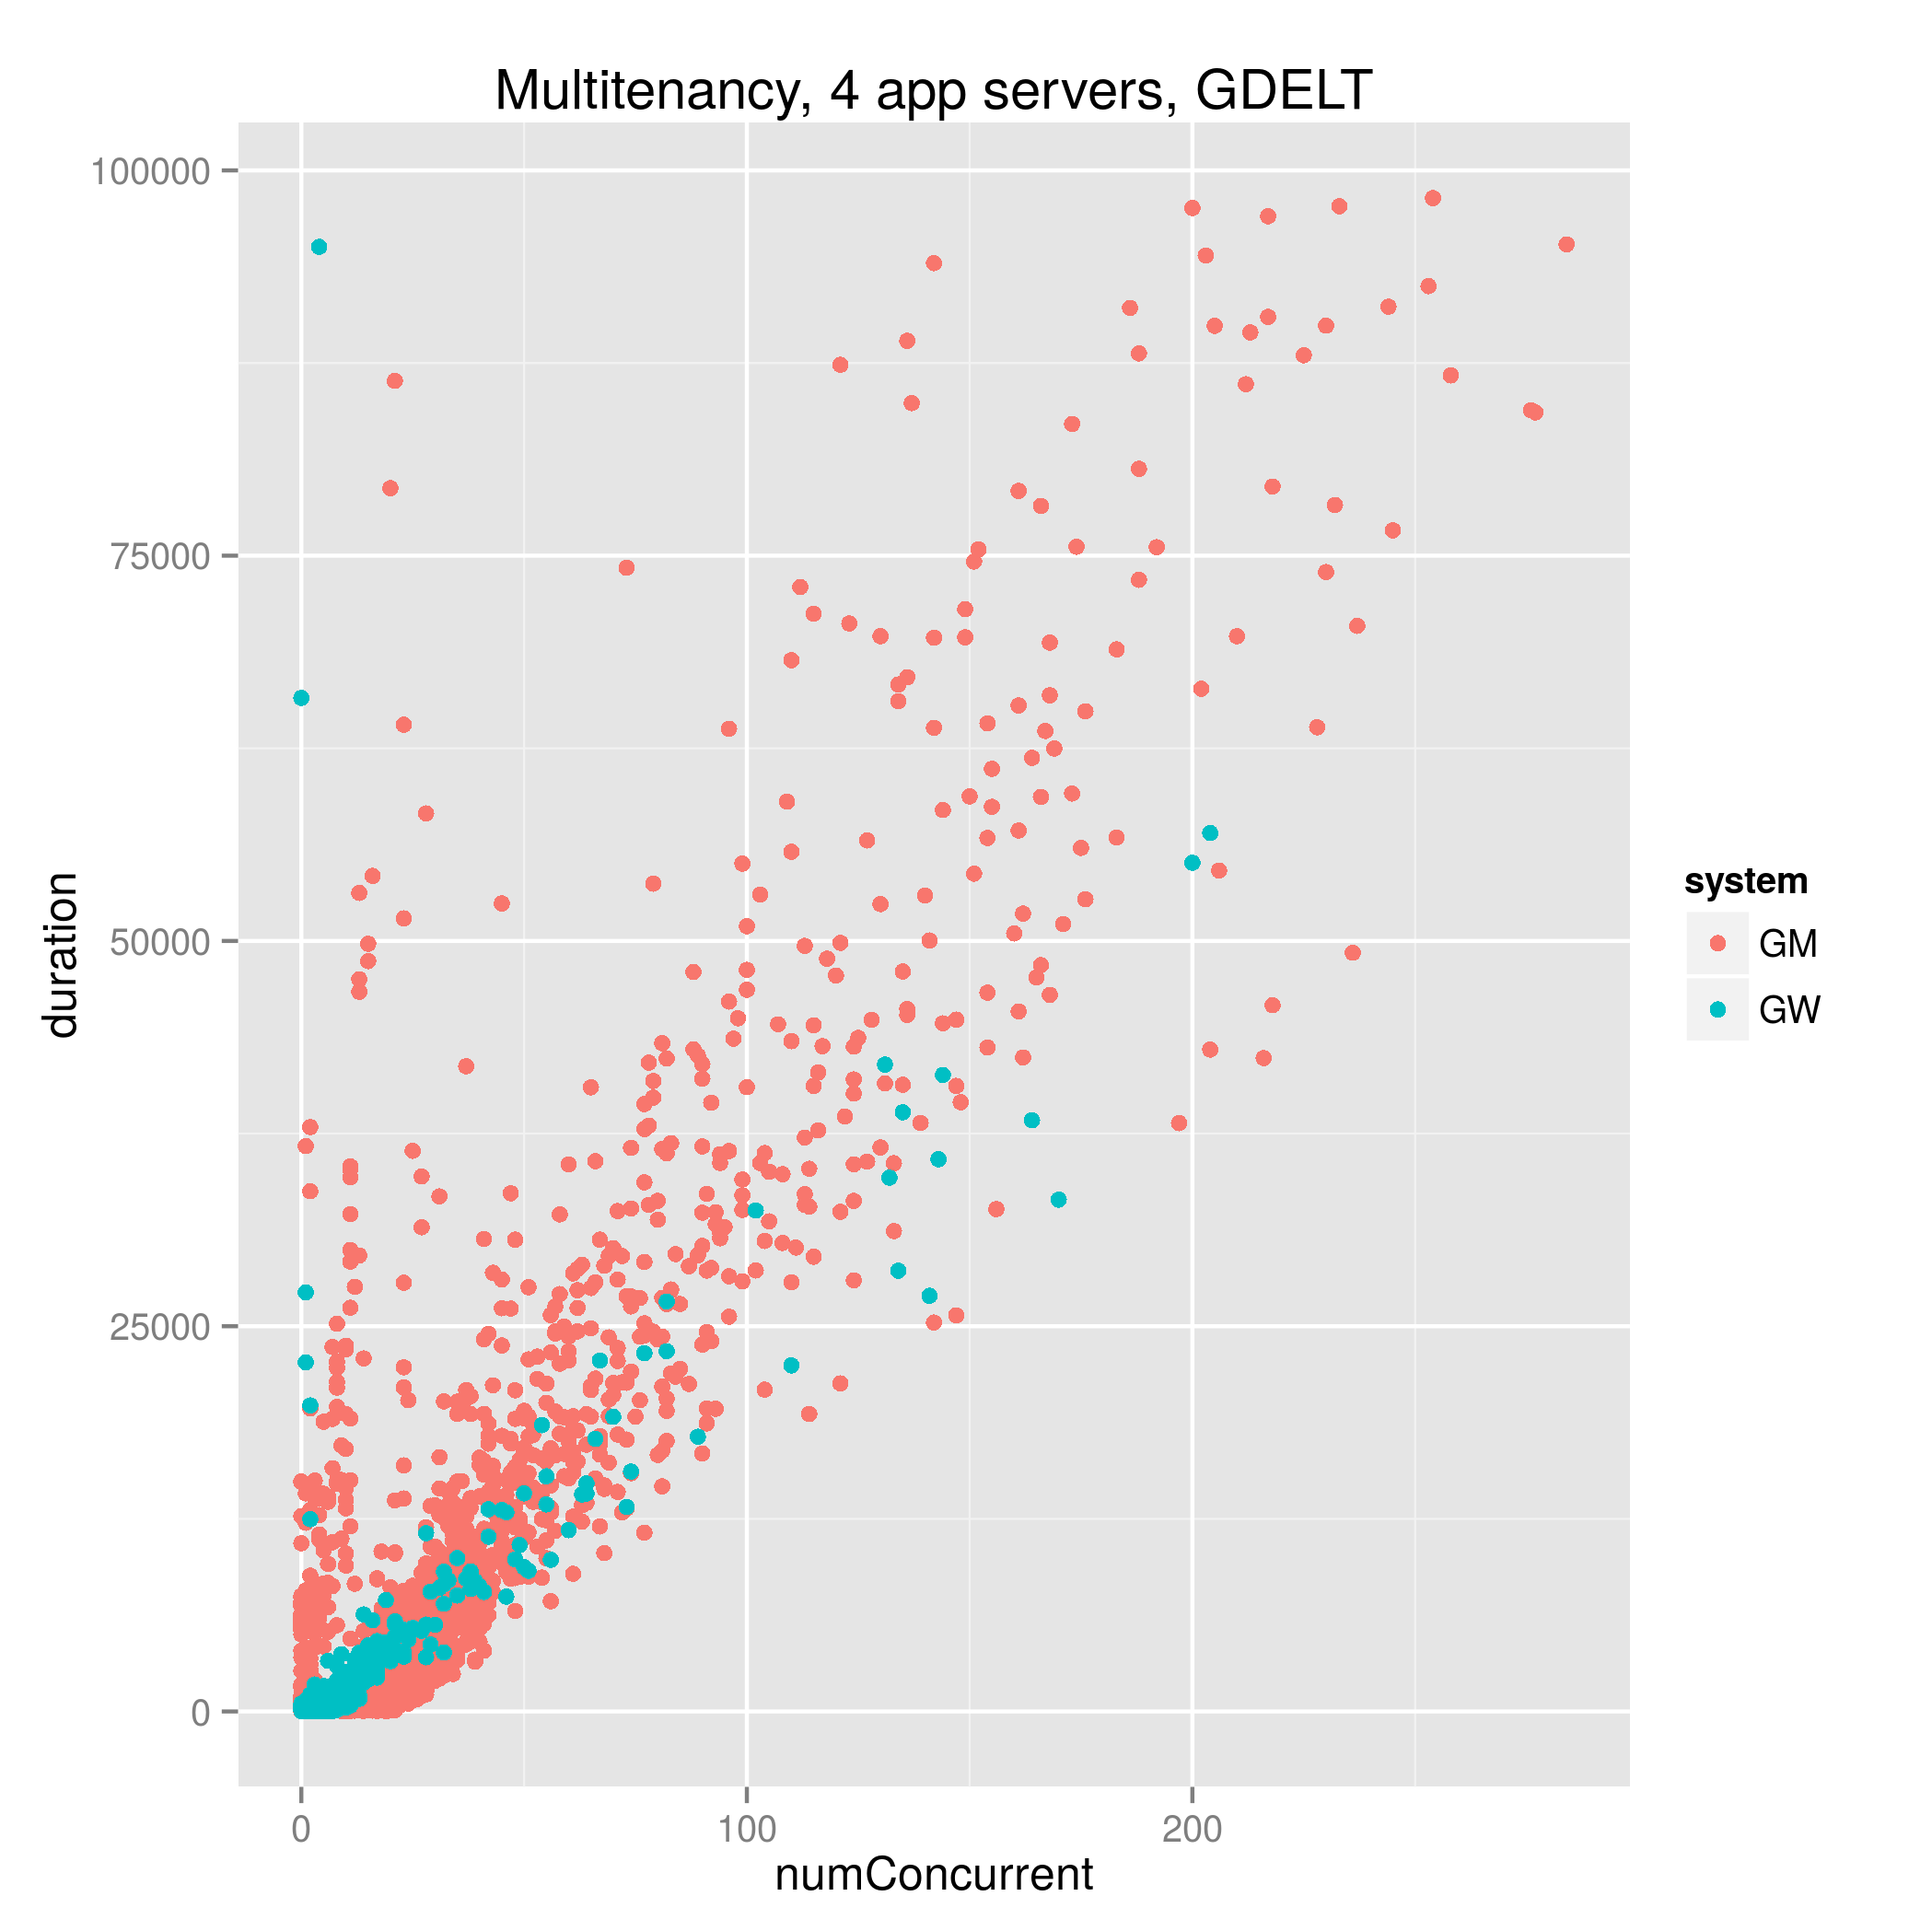
\includegraphics[width=0.60\textwidth]{../docs/img/multitenancy/graph_100k_mt2.png}
  \caption{Results for configuration 2.}
  \label{config2}
\end{figure}

{\bf Configuration 3: 6 Application Servers.}
We increase the application server count to six to verify that we have removed any performance impact from this parameter, as we expect the duration and concurrency distributions remain consistent, indicating that in both \texttt{MT2} and \texttt{MT3} results the cluster resources are the only remaining constraint.
However, at this point one of the two GeoMesa clusters started experiencing similar performance degradation as after \texttt{MT1} round of tests.
This can be seen as two distinct distributions of GeoMesa results.
\begin{figure}[h!tb]
  \centering
  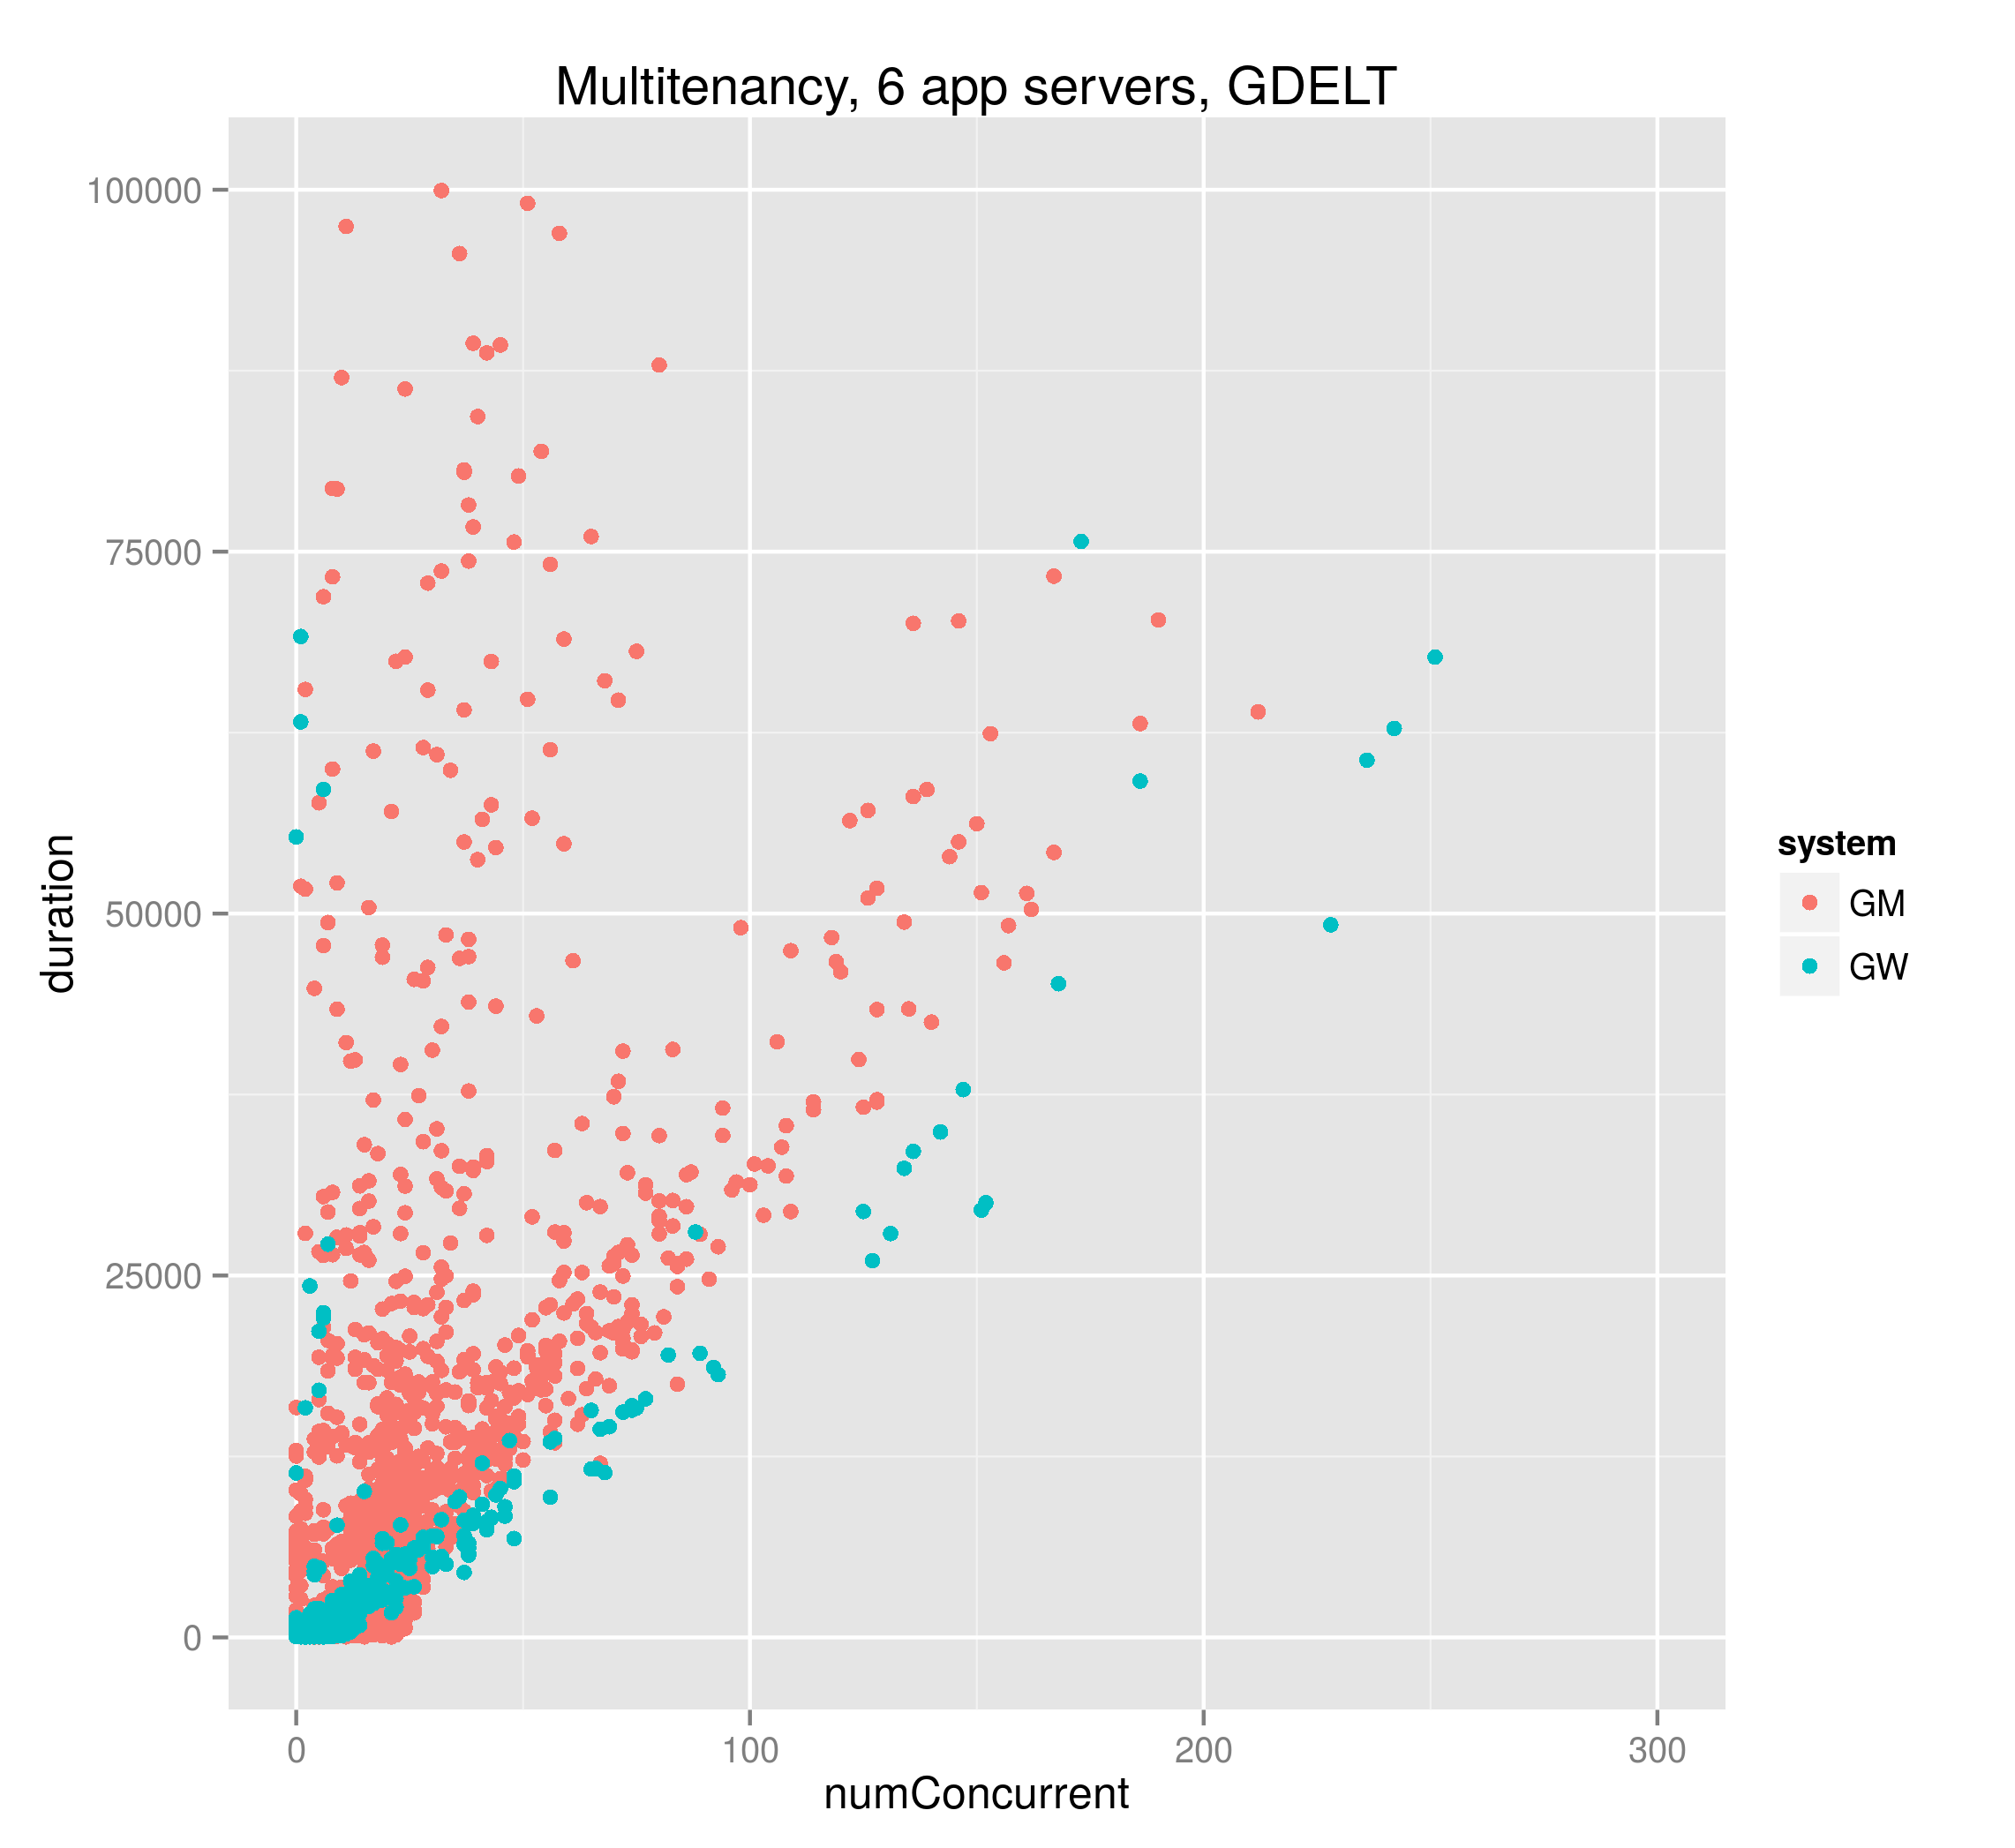
\includegraphics[width=0.60\textwidth]{../docs/img/multitenancy/graph_100k_mt3.png}
  \caption{Results for configuration 3.}
  \label{config3}
\end{figure}


\subsection{Synthetic Tracks Test Specifics}

This dataset is densest around continental United States and covers a single year, with track length biased to be short.
We project a powers of $2$ pyramid over this area and query from pyramid level $4$ to $8$ with temporal selectivity ranging from $5$ days to $1$ month.
The generated query requests are biased towards lower levels of the pyramid, proportional to the number of grid cells at each level.
We test initially with $16$, $32$ concurrent connections.
Because we have seen from previous tests that six application servers is sufficient to handle query load from our cluster we only test against this configuration.

\subsubsection{Test Results}

Increasing from $16$ to $32$ concurrent users produced nearly identical result counts per unit of time, $30$ minutes.
However, we see that it has increased latency for each request.

Most interesting are the response time distributions, which explain the difference in overall throughput.
GeoWave index trades minimum response time for more consistent and on average faster results.
Please see Figures \ref{geowave16}, \ref{geowave32}, \ref{geomesa16}, and \ref{geomesa32}.

\begin{figure}[h!tb]
  \centering
  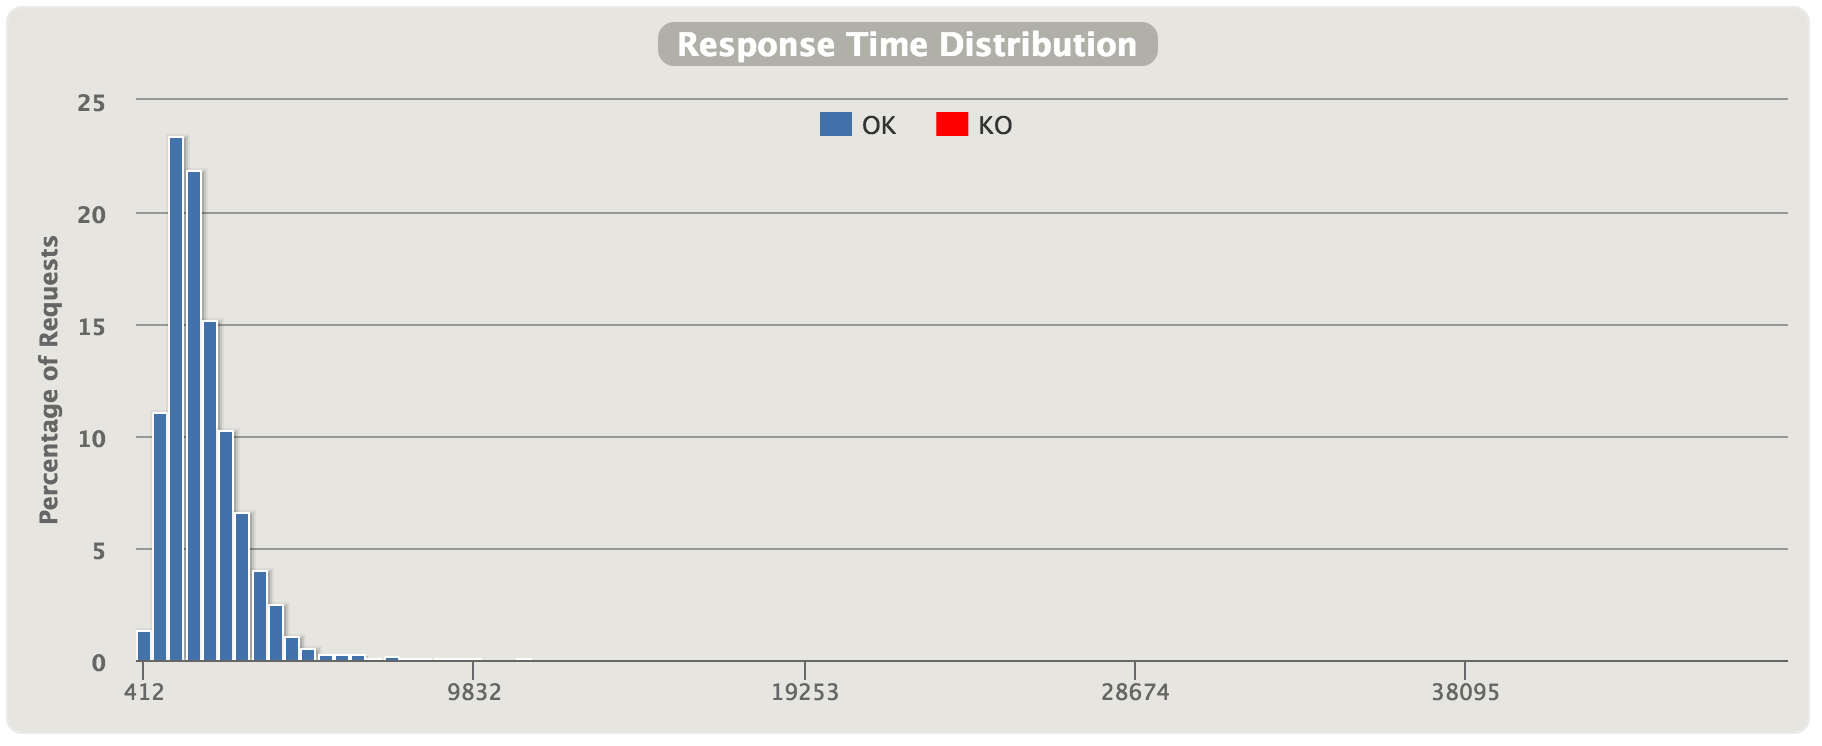
\includegraphics[width=0.60\textwidth]{../docs/img/multitenancy/gw-16-responses.png}
  \caption{GeoWave, 16 users.}
  \label{geowave16}
\end{figure}

\begin{figure}[h!tb]
  \centering
  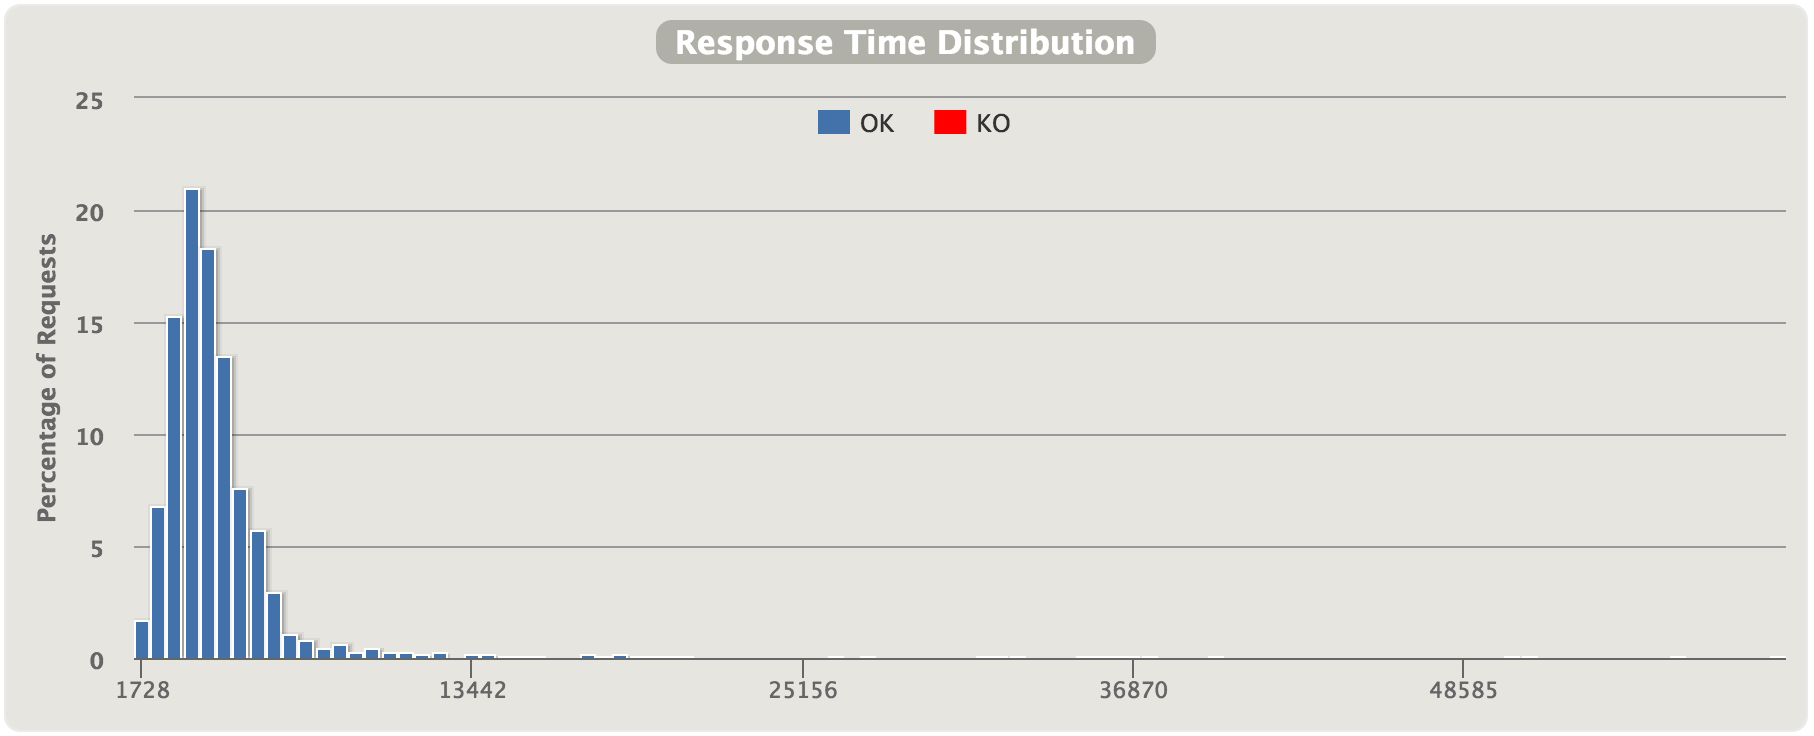
\includegraphics[width=0.60\textwidth]{../docs/img/multitenancy/gw-32-responses.png}
  \caption{GeoWave, 32 users.}
  \label{geowave32}
\end{figure}

\begin{figure}[h!tb]
  \centering
  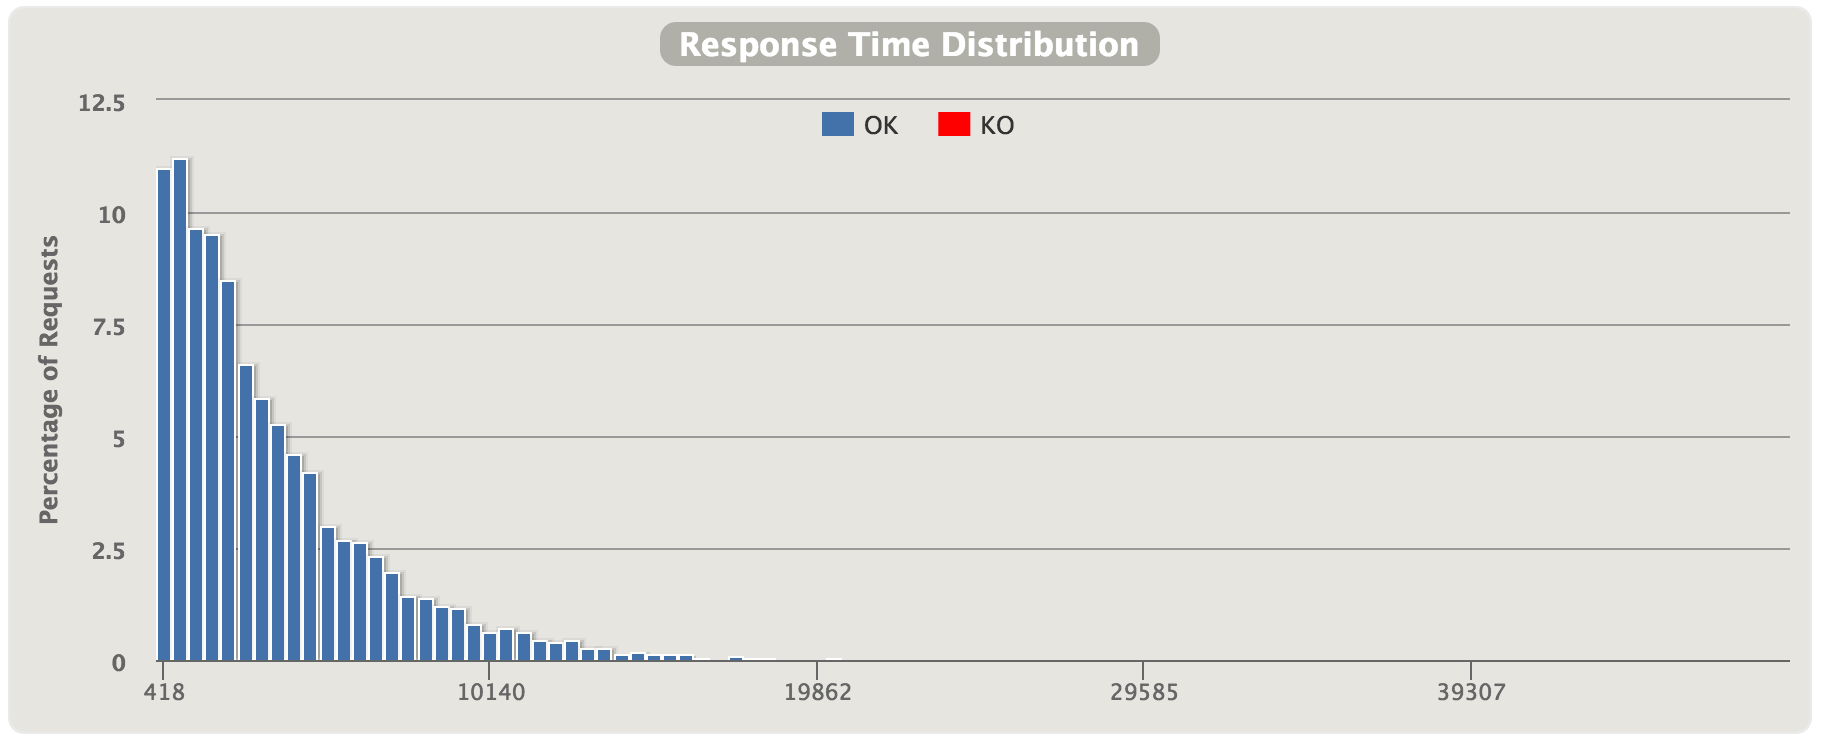
\includegraphics[width=0.60\textwidth]{../docs/img/multitenancy/gm-16-responses.png}
  \caption{GeoMesa, 16 users.}
  \label{geomesa16}
\end{figure}

\begin{figure}[h!tb]
  \centering
  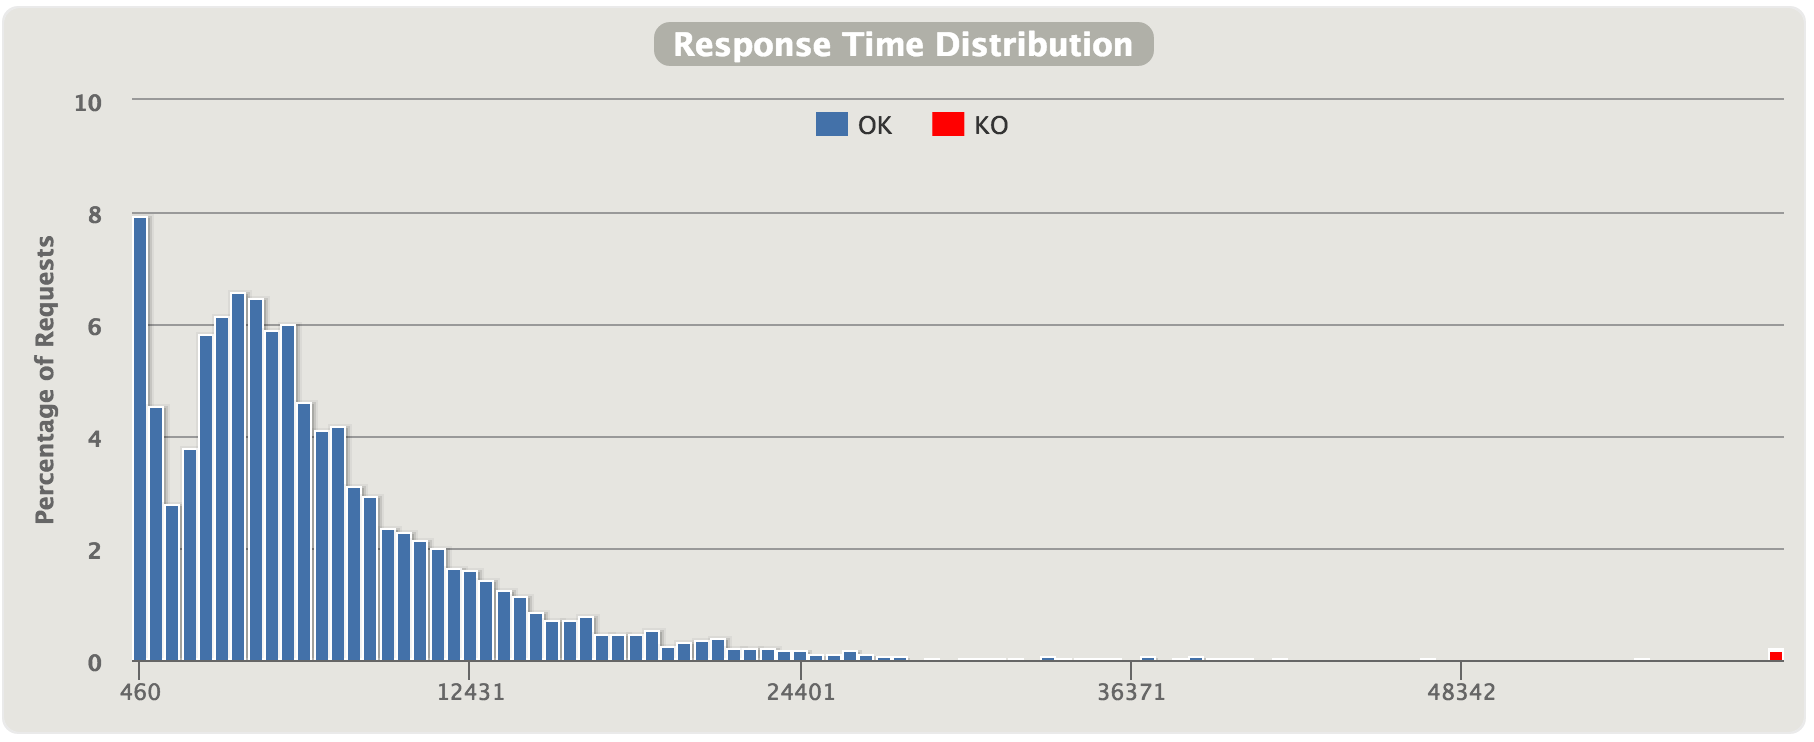
\includegraphics[width=0.60\textwidth]{../docs/img/multitenancy/gm-32-responses.png}
  \caption{GeoWave, 32 users.}
  \label{geomesa32}
\end{figure}
